\chapter{Introduction}
%labels will help you to reference to certain images, tables, chapters, section, and so on...
\label{introduction}
%DELETEME: for readability purpose, it makes sense to write a short paragraph on what the reader can expect in this chapter.
%
%DELETEME: tipp: sometimes it makes sense to write the first chapter, the last chapter, and the abstracts at the end. In this case, it might be easier to argue towards your topic

%%%%%%%%%%%%%%%%%%%%%%%%%%%%%% Deleted / Edited %%%%%%%%%%%%%%%%%%%%%%%%%%%%%%%%%%%

%requires us to stimulate less parts of the brain
%to operate a device is one step closer to intuition.
%Arguably, the human mind is highly dependent on voice as a stimulus \cite{voiceneurons}, which 
%and high-level way of communication among humans. Unlike operating sophisticated software on a computer or a hand-held device, a conversation usually does not require profound IT literacy due to a usually abstract graphical user interface (GUI) or the lack thereof in the case of a voice assistant. By depending on natural language in writing or voice and speech, the user is much less engaged with technical detail. On a market scale, this gives voice assistants today a competitive innovation advantage (CIA) for they are hence more accessible to more demographic groups. Arguably, the human mind is highly dependent on voice as a stimulus \cite{voiceneurons}, which makes us in turn process our ideas starting with an inner voice which translates easiest to words when we speak before it gets  ``funneled'' into actions \cite{alexapc18}

%IRRELEVANT: With evidence in fiction readings and Sci-Fi films, advanced human interaction with machines has always been an aspiration of the future \cite{businsider}., societies have shown an increasing tendency to avail technologies that make computers present in most domains of our daily lives. And though we still are far from it, we have come a long way in the recent years. With the boom of artificial intelligence and devices making high processing power a tangible option \textcolor{magenta}{statistic from graph about messenger surpassing social networks - Screen Shot 2017-11-19 at 17.15.18}


%%%%%%%%%%%%%%%%%%%%%%%%%%%%%% for later use %%%%%%%%%%%%%%%%%%%%%%%%%%%%%%%%%%%

%when it comes to. instinct.  at once. stipulate
% soundex
% for even more streamlined communication. 
% give impression/suggest can trigger and imaginary human the effect of being present
% average hits. astounding
%the problem that will be addressed.
% Both aspects are which. direct impact.
%what drives us to. guarantee. 
% prefer to at least get no information. 
% content. indicate. focal
% aspiration we long strove for . modelled . consist. once we gradually

% retrieval-based models - pursue - purpose - recognized / capacity -tangible
% shift - boom - however - niched - general purpose - predominantly
%in most new devices shipped in available
%  reaps - harness - enabling
% Therefore. and so forth. evidence 
% cognitive behaviour. backbone
% to technology, retaining a certain ranking within a business sector is influenced by trust. 


With over a third of the world's population projected to own a smartphone in 2018 \cite{statistasmartphones} and a substantial fraction thereof using smarthome gadgets and appliances on a daily basis, AI's role has become more interesting than ever in many disciplines including but not limited to productivity and entertainment.
Many technologies we take for granted today, such as dictation and word prediction, recommender systems or other digital analytics depend on Machine Learning and Natural Language Processing techniques that were only made possible thanks to the high computational power shipped in most devices gradually overtaking the consumer market.
This transition also facilitated the introduction of a new form of interaction through conversation with the hardware, paving the way to an aspiration modern societies have been striving globally \cite{Starwars}.
%%	- one option: besides Sci-Fi films; Her, Breakfast at tiffany's, Network
%%	- funnel towards Motivation...modularization and Einteilung of the paper
Whether in blockbuster 60s drama as seen in \href{http://www.imdb.com/title/tt0054698/?ref_=nv_sr_1}{``Breakfast at Tiffany's" (1961)} or in Sci-Fi romance in the movie \hypertarget{hermovie}{\href{http://www.imdb.com/title/tt1798709/}{``Her'' (2013)}}, an obsession with voice technologies is featured throughout from an answering machine on tape to a fully personalized but mass-produced voice-based operating system to even become a protagonist.\\

Conversational bots were already prevalent since the 80s in the form of Question Answering Systems based on query programming languages like PROLOG and SQL.
\href{https://en.wikipedia.org/wiki/ELIZA}{ELIZA}, considered as the world's first chatbot and though quite superficial as an NLP-based programme for psychoanalysis, already at its early stages demonstrated how humans can become emotionally attached to machines, transcending over the anomaly of making conversation \textit{not} with a human \cite{Weizenbaum1976}.
Today, combining ML with retrieval-based approaches allows a more advanced interaction with the system and yields smarter and more personalized conversations between man and machine.
Consequently, it is no longer a surprise that chatbots acquire social skills to make \href{https://en.wikipedia.org/wiki/Xiaoice}{Xiaoice}, the empathetic bot from China, possibly a new kind of friend made of silicon revoking the fiction element from \hyperlink{hermovie}{``Her''}.\\ 

So far, voice assistants represent an additional layer of abstraction from software beyond the graphical user interface (GUI) and are hence the closest we have come towards human communication.
They deconstruct another barrier between the user and the hardware as voice communication generally does not require profound computer literacy and the conversational models rely on our inherent ways of expression.
%%	- smalltalk f\"ahigkeiten\\ 
%%	- den menschlichen Aspekt suggerieren\cite{hiddenbrainpod}\\
%%	- menschliches Verhalten immitieren\\
As they simulate the human aspect and imitate its behaviour for instance with small-talk abilities\cite{hiddenbrainpod}, voice assistants are regarded as a convenience for daily tasks and are on their way to becoming a de-facto replacement to sophisticated actions we perform on the screen.
In fact voice searches now compose a large market segment with over a billion voice searches per month \cite{voicelabs:trends}
%\inote{\href{https://www.branded3.com/blog/google-voice-search-stats-growth-trends/}{check quality of statistics}}
and are predicted to make up about
``1 Billion Voice Assistant enabled devices in circulation by the end of 2018''\cite{voicelabs:trends} and 
30\% \cite{gartnerpreds17}\cite{searchblog}
of all searches by 2020 with currently highest rates coming from the youngest generations based on a survey\cite{globalwebindex} by Global Web Index. 
According to the Alpine.ai 2017 Voice Labs report there were 33 million voice-first devices in circulation in 2017 worldwide \cite{voicelabs} with tremendous shifts in number of units sold between 2015 and 2017.
This and more statistics hint at a revolutionary change towards our use as much as the introduction of the GUI and mouse were to the Command Line Interface (CLI).
Increasingly, we recognize voice as a \textit{new} user interface, also known as Voice User Interface (VUI), and analyse good practices and design guidelines for it.\\

Since sound and voice are primal stimuli in the human brain \cite{voiceneurons}, using them becomes more instinctive, making us in turn process our ideas starting with an ``inner voice'' that translates easiest into words when we speak it before routing or ``funneling'' it to actions \cite{alexapc18}.
Arguably, on a market scale, this gives voice assistants today a competitive innovation advantage (CIA) for they are hence more accessible to further demographic groups with a growing wider acceptance.\\

Meanwhile, statistics from BusinessInsider \cite{businsider} show that time spent on messaging applications (apps) already surpassed average uptime on social media, which indicates how the former is more desirable as a communication format on mobile platforms and how having a conversation is an easier way to interact with a device instead of downloading an app for every task. %\inote{link ok?}
Further, the speech-to-text/text-to-speech domain has become more powerful with steadily increasing processing power, an effect of Moore's law we only get to understand lately in addition to the gradual lessening of the dominance of Chomskyan theories of linguistics (e.g. transformational grammar) \cite{wiki:nlp}.
With an integration in most modern operating systems, speaking to a device has become no longer a absurd novelty. 
Inadvertently, the Google voice assistant built into its Android OS currently with the highest usage shares among computer and smartphones \cite{wiki:gartnerreports}, supports understanding of multiple languages in the same sentence for multilingual interaction. %not going to call it google now since it's an ambiguous name
Moreover, the Echo Dot recorded the peak for best-sellers for 2017 on Amazon with unprecedented numbers showing a high customer retention and satisfaction rate \cite{cnbcAlexa}\\

%	- imagination about ablitiy to react to everything\\
As we constantly challenge our expectations towards technology, our imagination makes us question the ability of AI to make a machine able to react to everything we say, which can be not too far-fetched in a near future.
Although we are still far from this step, at least for the consumer level, we dedicate a lot of effort to make it happen with examples like IBM's Watson or other Uses of big data analytics.
We can probably conclude though, that as long as we still do not exactly understand human intelligence in detail yet, it is hard to fathom AI as a holistic field. As such, it is therefore more realistic to consider the current works in the field as \textit{intelligence amplification} \cite{alexapc18} empowering human take better decisions beyond their normal brain processing power and not overtaking human intelligence as some might claim.
\\

%###################################################################################
%###################### 	Motivation      ########################################
%###################################################################################
\section{Motivation}
\label{motivation}
%DELETEME: This section is very important since it argues why it is necessary to take care of the problem you are addressing in your work. One way to do this is coming from a very broad view on the problem to a very detailled one. This can be done by establishing a chain of statements that refer to each other until you reach your particular problem. Doing this, you really need to take care for citing every statement.

%DELETEME: Example for a chain: Mobile communication gets increasingly popular in the world (CITE sales on mobile communication infrastruce, mobile phones, or increasing number of mobile phones contracts). $\rightarrow$ Especially smartphones, which represent the next generation cellular phone (CITE), get more and more used for communicating not only with other people but also for connecting to the Internet for using various services (CITE). $\rightarrow$ Smartphone are comprehensive cellular phones that additional functionality due to their increased connection and processing capabilities (CITE). $\rightarrow$ Most smartphones offer an online application store for adding software to the devices which helps the users to customize their devices according to their needs, e.g. Android Market\footnote{\url{http://market.android.com}, visited on 05/08/2011}. $\rightarrow$ One problem about installing third-party software is that not all softwares try to help the user; $\rightarrow$ software with malicious intentions, so called malicious software (malware), can be a severe threat to smarpthone users. Some malwares delete files (EXAMPLE + CITE or footnote with URL) or even destroy devices (EXAMPLE + CITE or footnote with URL). $\rightarrow$ More and more smartphone malwares appeared in the last years (CITE). $\rightarrow$ Signature-based approaches work efficiently on known malware (CITE) but face serious drawbacks regarding unknown malware. $\rightarrow$ Oberheide et al.~\cite{oberheide:2008:cloudav} state that virus engines need an average time of 48 days until their databases get updated to be able to detect a certain unknown malware. $\rightarrow$ This in turn means that smartphone users stay unprotected for this time which can be seen as a severe threat. $\rightarrow$ Therefore, approaches are needed that are capable of detecting unknown malware for protecting the users against such threats.
%DELETEME: This example showed how one could argue that alternative approaches for malware detection is required. The length of the motivation depends on the topics handled and can of course be longer. The principle I am describing is also shown on Figure~\ref{fig:writing}

%%%%%%%%%%%%%%%%%%%%%%%%%%%%%%%%%%%%%%%%%%%%%%%%%%
%% why bots:juxtaopse human to machine etc - biased pros/cons
%
%%- unfortunately forums and FAQ pages are not as effective as talking to a human.\\ 
%%- then again, as a customer, if I want assistance, I want the customer to tell me related information that he/she might not know, e.g. model number etc.\\
%%- making the bot become something beyond a Q\&A:\\
%%%%%%%%%%%%%%%%%%%%%%%%%%%%%%%%%%%%%%%%%%%%%%%%%%
With the aforementioned, we try to think how voice assistants could come handy and why we want to invest in such technology, juxtaposing it to available alternatives.
If we consider human workforce (i.e. customer service agents) on one hand, it is commonplace that these are more expensive, less available due to restrictive working hours and not always aware of the full circumstances related to an issue they are supposed to fix or a question they are to answer. 
%%%%%%%%%%%%%%%%%%%%%%%%%%%%%%%%%%%%%%%%%%%%%%%%%%
%- besides, I could be a bit more sure in customer support scenario that a bot won't trick me\\
%- what bots already achieved is at least not to give wrong answers.\\
%%%%%%%%%%%%%%%%%%%%%%%%%%%%%%%%%%%%%%%%%%%%%%%%%%
Sometimes knowing more about a person could almost become a dangerous tool since it gives room to manipulate them. 
A client in a shop for instance can have their decision influenced by the seller and eventually get tricked into buying a product based on wrong advice.
Although there is practically little the client can normally do to circumvent misinformation if that seller is replaced by an algorithm, having an automated system like a voice assistant step in gives at least a more neutral impression since it are not directly expected to act with malicious intentions like a vendor who abuses the client's trust.\\

%%%%%%%%%%%%%%%%%%%%%%%%%%%%%%%%%%%%%%%%%%%%%%%%%%
%- they could sometimes say idk, which is annoying, but at least it doesn't confuse the user.\\
%%%%%%%%%%%%%%%%%%%%%%%%%%%%%%%%%%%%%%%%%%%%%%%%%%
Since the point of availing voice assistant is to act in a person's interest, we also want an information system not to confuse us or to limit our cognitive abilities.
%\inote{talk about cognitive behaviour}
Besides, we can at least ensure in a system design that a voice assistant will not become moody and intentionally want to make our lives harder for this reason as opposed to a human.
And so, although a voice assistant or a chatbot may not potentially answer every question we throw at it, we want to at least presume that it would give us no information instead of partial truths or lies while keeping a certain level of neutrality and ``decency'' in terms of the wording.
%%%%%%%%%%%%%%%%%%%%%%%%%%%%%%%%%%%%%%%%%%%%%%%%%%
%talk about this in design section: bot muss höflich sein, we can get angry at it, it should still remain 'unsentimental'
%%%%%%%%%%%%%%%%%%%%%%%%%%%%%%%%%%%%%%%%%%%%%%%%%%
This is why most credible companies elaborate explicitly in their terms, conditions and privacy statements on what makes them accountable on the %products they produce and 
the services they offer.
A consumer therefore feels more empowered to assert any faults originating from an automated system than from a human and conditionally has an assurance that they can prevent any violations more systematically.\\

Eventually a person is more likely to develop a certain kind of trust in a machine more than in a human once the technology is established and widespread.
Cars, email, and other gadgets or services we take for granted today are living proof of how inevitably this trust grows, for the better or worse and depending on the degree of affinity to the related technology, aversion or ignorance in a business sector.
Trust in a system can grow once it is certified to have little to minimal exceptions. Besides enriching the value chain, it is a key in setting a technology to become an industry standard.
Therefore, if a voice assistant is shown to deliver reproducible results disregarding a person's profile, this definitely contributes towards the credibility of the system.
This is however not an easy case, since an advanced voice assistant is not expected to be deterministic in most situations, otherwise it becomes boring! We elaborate later in this thesis how %utterances~\tocite{} 
we handle this problem.\\

%%%%%%%%%%%%%%%%%%%%%%%%%%%%%%%%%%%%%%%%%%%%%%%%%%
%- as a novice I am usually not sure if the help article / Kbase I am reading is the right one\\
%- and forums have mostly Schrott anyway.\\
%%%%%%%%%%%%%%%%%%%%%%%%%%%%%%%%%%%%%%%%%%%%%%%%%%
On the other hand, Information Retrieval Systems range from web pages (e.g. frequently asked questions section (FAQ), forums or a search engine). These are in some cases even less effective than contacting a human as getting the proper information takes a lot of time, or the level of trustworthiness or participation levels in a forum are particularly low, the problem stated is too broad or too specific compared to the answer we are seeking. A user also could come unintentionally across false positives in a search and rely on irrelevant information without knowing.
Furthermore, some case-related information might be required to have a proper understanding of a situation or a scenario and provide adequate answers. For Example, if a user would like to know if a certain accessory is compatible with their mobile device, they might need to give a model number, which they may or may not know.
Consequently, it is of high interest to maintain a system that could determine all these factors autonomously or with the least possible human interference such that a system supersedes the abilities of the classical Q\&A approach.\\

%%%%%%%%%%%%%%%%%%%%%%%%%%%%%%%%%%%%%%%%%%%%%%%%%%
%- use of translators, Stammsprache, etc., detecting the language and say it does not support it.\\ 
%- internationalization / customization based on Locale
%- why is it important?\\
%- many international users prefer a chatbot than a phone since the bot will communicate more accurately, will not have language problems if it understands the foreign lang etc.\\
%- what are other approaches to localization? refer to IRS lecture notes\\
%- for facebook: implementing the three-answer suggestions to help user know what they say or alexa etc
%%%%%%%%%%%%%%%%%%%%%%%%%%%%%%%%%%%%%%%%%%%%%%%%%%
Internationalization is also another factor to take into account. Since languages differ not only in their vocabulary but also grammar, word and sentence structure (e.g. false friends, nuances, phrases, idioms), developing a voice-first device requires a flexible infrastructure and software stack both able to accommodate these deviations.
In that respect, not only is region-specificity important, but also being able to cater for people in a region who do not speak its official language or are residing there temporarily.
Especially in businesses where it's difficult to hire skilled foreign-language speaking personnel, a voice assistant can overcome this challenge as it would communicate more accurately and will not have language problems.
The customer is then given the option to avoid an inconvenient experience with the typical scenario with a call centre representatives where neither of both parties understands the other.
For those who have minimal understanding of the language, there are possibly also options to provide help in the native language if the user is given the options he/she can answer a prompt with. At the very least, a VUI could still give feedback to the user of wether it understands the language or not, since algorithms for detecting a language are not as complex as answering the question once the language and its dialect (also known as locale) is deciphered. %understood.
All of which are optimal use cases for ML approaches and algorithms such as term weighting discussed in Section \ref{discussions} based on simpler approaches to localization from an original text, such the corpus-based mapping approach. WordNet is one such example. %Auch: Stammsprache,...refer to IRS lecture notes
Finally, giving the user clues on what to answer with is also a helpful tool, as we will also discuss in bot design (Chapter \ref{mainone})



%%%%%%%%%%%%%%%%%%%%%%%%%%%%%%%%%%%%%%%%%%%%%%%%%%
%%%%%%%%%%%%
%%%%%%%%%%%%%%%%%%%%%%%%%%%%%%%%%%%%%%%%%%%%%%%%%%
\section{The Analyzed Scenario}
\href{https://www.berlin.de}{Berlin.de} is an online one-stop-shop for approximately 3,7 million residents of the German capital\cite{zensus} with thousands of visitors daily for information lookup, appointment bookings and even access to local news.
%on its website
%and particularly a few hunderds of which are users of the Virtual Citizen Assistant.
As part of a federal modernization procedure with the help of the German Ministry of Interior, D115 was launched in 2009 \cite{d115} as a phone service to help residents find relevant information about a public service or municipality, something that can be tricky if a person has no overview of the local government structure and still not always easy even with the help of search engines nowadays with the array of public services provided.
To promote information accessibility, D115 continuously aims at expanding its reach and services.
It is therefore worth exploring, how to offer D115 services in a fashion that takes advantage of conversational abilities beyond its human personnel or online city portals. 
\\

%%%%%%%%%%%%%%%%%%%%%%%%%%%%%%%%%%%%%%%%%%%%%%%%%%
% the language barrier could be even more frustrating. This is where a chatbot could step in, acting as a mediator that can translate natural language into a query for lookup.
%%%%%%%%%%%%%%%%%%%%%%%%%%%%%%%%%%%%%%%%%%%%%%%%%%
For now, although local authorities rely heavily on their websites to communicate information to the public, the challenge is mainly finding the right service even with an vague query since most of the time a person requesting a public service is not fully aware of the exact service name in the catalogue of services offered or cannot differentiate between two similar public services or even know if one of them is required in their case.
In a metropolis with a high influx of incomers, it is also very likely that certain services are frequently pursued, meaning that helping find the right public service or authority is a repetitive task. In this context, thinking of a voice assistant as a public service could have several advantages, like offloading some traffic from the phone service, getting over the language barrier in the case of non-German speakers, expatriates or simply helping native customers formulate the right wording for a query in a more intuitive way than using a search box. 

%%%%%%%%%% could still be included %%%%%%%%%%%%
% on the other hand more and more people ``trust" new technologies and the trends like social media, bots, selfies .. ripple effect - normaization -> results of data collected, what we know about people more than ever before

% like listing required documents for a service, addresses of where the service is offered with opening hours and report on the legal basis of a serv. 

% between how a person can express his their guidance in 
% there are also several 
% Provided that one understands
% for confused customers
% thoroughly aware - desired
% with the aforementioned techniques, such functionality becomes possible\\
% ~~~~ few things are lost here! many things thanks to git!!



%%%%%%%%%%%%%%%%%%%%%%%%%%%%%%%%%%%%%%%%%%%%%%%%%%
%service bots for the public
%further service continue to expand to cope with even newer trends.\\
%%%%%%%%%%%%%%%%%%%%%%%%%%%%%%%%%%%%%%%%%%%%%%%%%%
All of which leads to thinking how providing voice assistants and/or a chatbots for public services could make us reap the benefit of available technologies and extend it aiming for continuous modernisation of our connected living to blend into a seamless digital lifestyle \cite{dai:cl}. 






%###################################################################################
%###################### Approach and Goals  ########################################
%###################################################################################
\section{Approach and Goals}
%DELETEME: In this section, you should cleary describe your approach that you are following in order to solve the underlying problem of your thesis. Additionally, you should clearly state the goals of your work. This will not only help you supervisor to understand what you are doing, it will also help you to be sure on which topic you should evaluate.



%%%%%%%%%%%%%%%%%%%%%%%%%%%%%%%%%%%%%%%%%%%%%%%%%%
%\todo{\textbf{Aufgabenstellung:}\\ 
%	-AL: Anschlie{\ss}end soll das Ziel der Arbeit formuliert werden: Entwicklung und Evaluation eines Prototypen f\"ur den Anwendungsfall.\\
%	\\
%	1- es sollen die St\"arken und Schw\"achen eines solchen System zu analysieren. 
%	2- Es sollte zun\"achst eine Dienstleitung aus dem Berliner Service-Katalog mit dem Chatbot \"beauskunftet\" werden k\"onnen.\\
%	3- Nuancen beachten (e.g. 10243 / FHain)\\
%	4- Smalltalk F\"ahigkeiten
%}
%%%%%%%%%%%%%%%%%%%%%%%%%%%%%%%%%%%%%%%%%%%%%%%%%%
%\inote{refactor}
In the following thesis, we take these factors into consideration and narrow them down to fit our tailored scenario in the e-Government sector. We start by surveying industry-standard %prominent 
voice assistants platforms like Siri, Bixby, etc. and frameworks such as Microsoft Azure Bot Framework, Amazon Lex and API.ai,
and present a solution that caters for the local municipality of Berlin, Germany.

For this we choose to present our solution using Alexa based on our criteria in Section \ref{choiceOfPlatform}.

With an agile approach, we present functional code for running and deploying the aforementioned service on Amazon's voice assistant through a so-called ``Alexa Skill'' and analyse the strengths and weaknesses of choosing this platform. We start by exploring the available public services on \href{https://service.berlin.de}{https://service.berlin.de} 
to understand how to implement our Skill. 
We then choose a set of examples with different levels of implementation difficulty to prototype how all current and future \href{https://service.berlin.de}{Berlin.de}'s 
services should be handled using knowledge from existing databases.
Difficulty is expressed in the required knowledge of the Skill to perform a user's request. \inote{This includes for instance abilities like the system to understand the district location intended by the user through a postal code input.}

Further, we test the Skill using unit tests for the code and usability tests for the interaction model especially with the ability to identify and deal with.
In the code, we alread have the advantage of many small-talk abilities since we build on top of Alexa's existing and continually expanding database for question-answer models.
\inote{mention that this could get you out of the skill in the pro/con section.}

\sn{besser ganze Sätze,bullets tamam}
In summary, these goals were defined for the system:

\begin{itemize}
	\item understand user's requests about public services through different sentence formulations
	\item deliver relevant information based on the service requested
	\item communicate with an endpoint that builds on the service catalogue of Berlin.de's ``Virtueller Bürgerassistent''
	\item produce a scalable, modular system that can be extended in the future
\end{itemize}

Further requirements are discussed in Chapter~\ref{mainone}.






%%%%%%%%%%%%%%%%%%%%%%%%%%%%%%%%%%%%%%%%%%%%%







%\begin{figure}
%\centering
%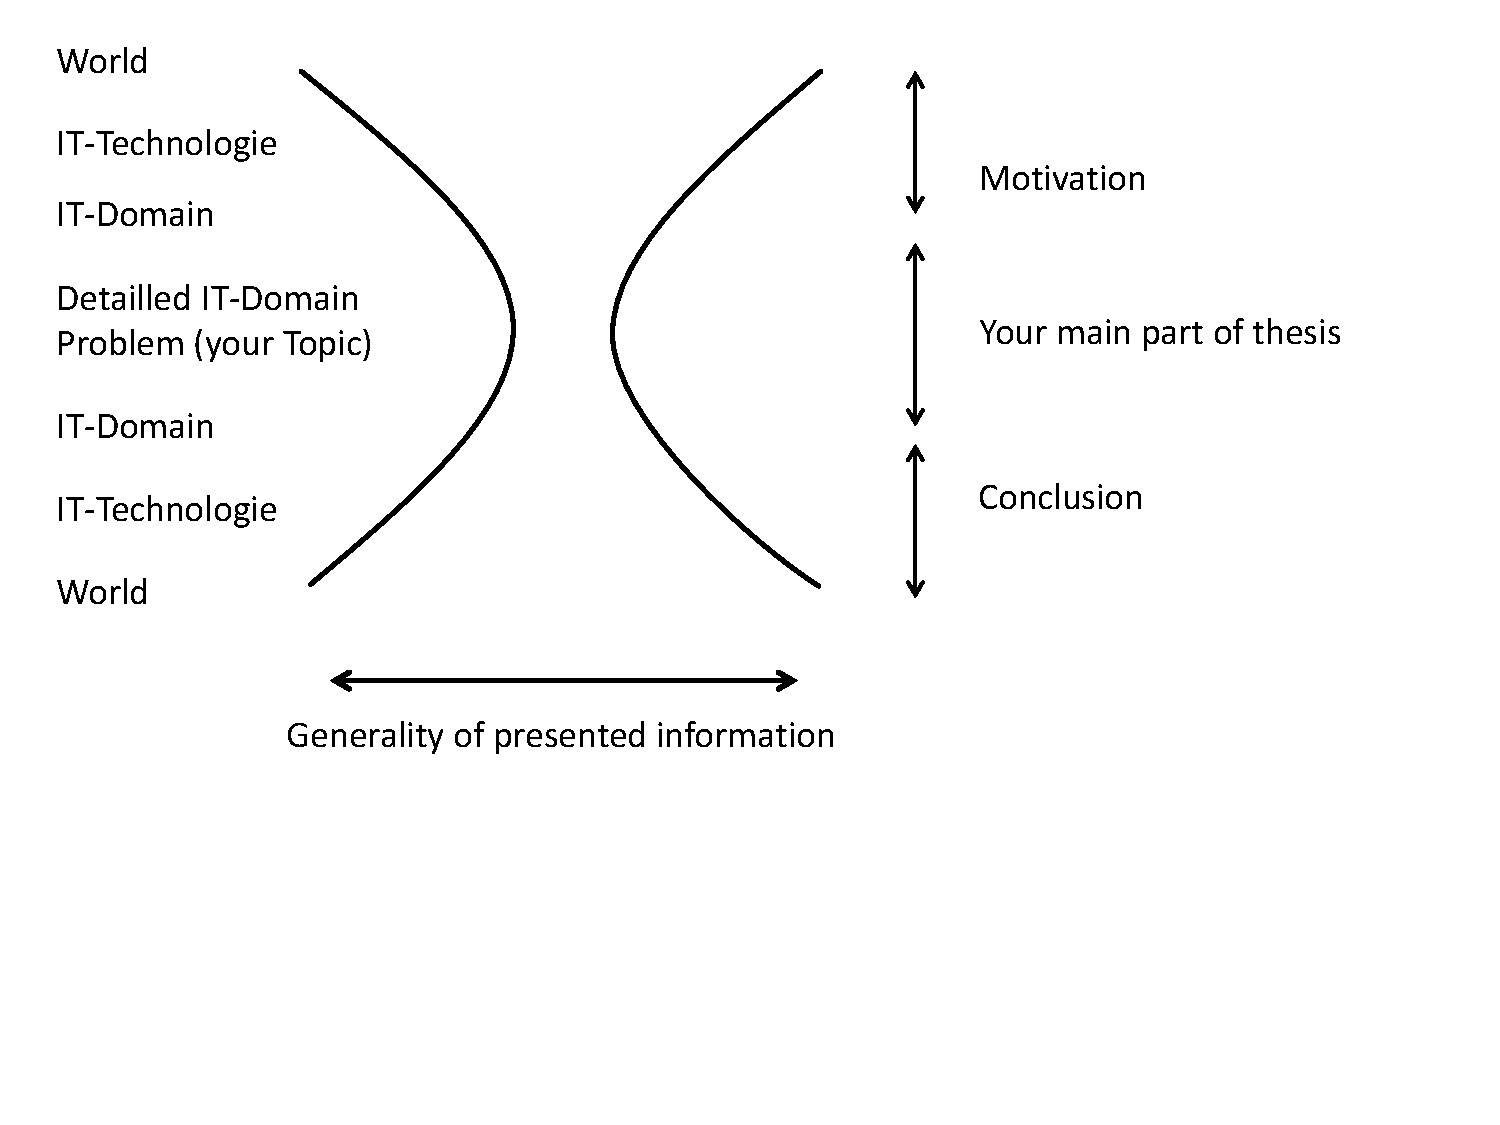
\includegraphics[width=0.9\textwidth]{template/writing}
%\caption[Information Generality]{This images illustrates how generality of information could be handled in a thesis. In your motivation you should start from a very broad view on the topic. Then you should get more precise with every statement until you reach the actual problem you are addressing. You should do vice-versa in your conclusion, starting with the problem that you addressed and getting broader until you can write about the meaning of your results to the (IT-)world.\label{fig:writing}}
%\end{figure}









%###################################################################################
%###################### Structure of the Thesis ####################################
%###################################################################################
\section{Structure of the Thesis}
%DELETEME: This section does not require eloquent writing. It is just a presentation of what you will handle in each chapter starting with Chapter~\ref{background}.
%

%This thesis endeavours to shed light on the following: 
This thesis is organised as follows:
In Chapter~\ref{background}, 
we first introduce in section \ref{choiceOfPlatform} the available platforms and explain why we choose Amazon, going over the idea behind Alexa Skills.
% then discuss related work as currently available. Going beyond 
From there in section \ref{relatedWork} we show some related work according to our use case in the public sector %we show a few comparative %exemplary
%implementations for 
%in the form of a chatbot and a voice assistant in English- and German-speaking context. 
for Vienna, Austria and Georgia, USA.
We compare them to the current chatbot application ``Virtueller Bürgerassistent'' available on \href{https://service.berlin.de/virtueller-assistent/virtueller-assistent-606279.php}{service.berlin.de}, which we build our work on with the same underlying technology using Apache Solr.

%for German and Singapore/ \href{http://www.govtech.com/7-State-or-Local-Governments-Using-Amazon-Alexa.html}{LA/...} for English} 
In Chapter~\ref{mainone} we introduce our design to the Skill and discuss how it 
%can overcome a few struggles with respect to 
addresses
redundant boilerplate code, smalltalk abilities and briefly highlight some limitations on the system limitations. We also present the frameworks and Application Programming Interfaces (APIs) we use in our own implementation, the prerequisites and the artefacts provided initially through a breakdown into several cases simulating common uses on Berlin's city portal.


%its counterparts \inote{like , , but also limitations}. 
Chapter ~\ref{maintwo} 
%represents a detailed analysis of 
explains our implementation solution. We elaborate in particular on how we deal with individual public services in the interaction model from front-end and back-end perspective, how we connect the web services together and analytically document the code structure, endpoints in addition to the deployment process. The related code is available on \href{https://www.github.com/megantosh/AlexaImAmt}{GitHub} \footnote{\url{https://www.github.com/megantosh/AlexaImAmt} \todo{make sure this is final URL and is public before printing}} with a digital copy attached to this work. 

Chapter~\ref{evaluation} evaluates our implementation with respect to our target in the defined %\inote{4-5} 
use cases. We base our evaluation models on a survey we conduct that helps us specify requirement details, as well as automated tests provided by the framewor we use in addition to usability, performance and unit tests. 

In Chapter~\ref{conclusion}, we conclude the work focusing on how our implementation %of this e-Government solution 
is attainable through Alexa and where future works can be directed for an e-Government solution.
%Chapter~\ref{appendices} gives additional related information on the topic of this thesis.}
%to head